\documentclass[11pt,fleqn]{article}
\usepackage{../cs70,latexsym,epsf,amsmath,amsfonts,amssymb,graphicx,url,polynom}

\lecture{8}
\def\title{Note \the\lecturenumber}
\begin{document}
\maketitle




\section*{Polynomials}
Polynomials constitute a rich class of functions which are both easy to 
describe and widely applicable in topics ranging from Fourier analysis
to computational geometry. In this note, we will discuss properties of polynomials
which make them so useful. We will then describe how to take advantage of these
properties to develop a secret sharing scheme. 

Recall from your high school math that a {\it polynomial\/} in a single
variable is of the form $p(x) = a_d x^d + a_{d-1} x^{d-1} + \ldots + a_0$.
Here the {\it variable\/} $x$ and the {\it coefficients\/} $a_i$ are usually 
real numbers. For example, $p(x) = 5x^3 + 2x + 1$, is a polynomial
of {\it degree\/} $d = 3$. Its coefficients are $a_3 = 5$, $a_2 = 0$,
$a_1 = 2$, and $a_0 = 1$. Polynomials have some remarkably simple,
elegant and powerful properties, which we will explore in this note.

First, a definition: we say that $a$ is a {\it root\/} of the polynomial 
$p(x)$ if $p(a) = 0$. For example, the degree $2$
polynomial $p(x) = x^2 - 4$ has two roots, namely $2$ and $-2$, since
$p(2) = p(-2) = 0$. If we plot the polynomial $p(x)$ in the $x$-$y$ plane,
then the roots of the polynomial are just the places where the 
curve crosses the $x$ axis:

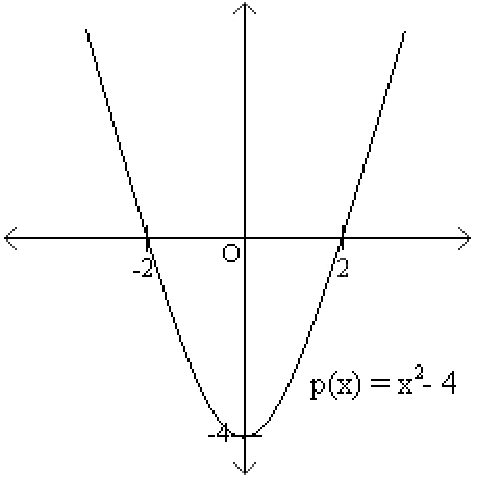
\includegraphics[bb = 0 0 140 240, scale = .5]{quad}


We now state two fundamental properties of polynomials that we will prove
in due course.

\noindent
{\bf Property 1:} A non-zero polynomial of degree $d$ has at most $d$
roots.

\noindent
{\bf Property 2:} Given $d+1$ pairs $(x_1, y_1), \ldots, (x_{d+1}, y_{d+1})$,
with all the $x_i$ distinct, 
there is a unique polynomial $p(x)$ of degree (at most) $d$ such that
$p(x_i) = y_i$ for $1 \leq i \leq d+1$.

Let us consider what these two properties say in the case
that $d =1$. A graph of a linear (degree $1$) polynomial 
$y = a_1 x + a_0$ is a line. Property $1$ says that if a 
line is not the $x$-axis (i.e. if the polynomial is not $y = 0$), 
then it can intersect the $x$-axis in at most one point. 

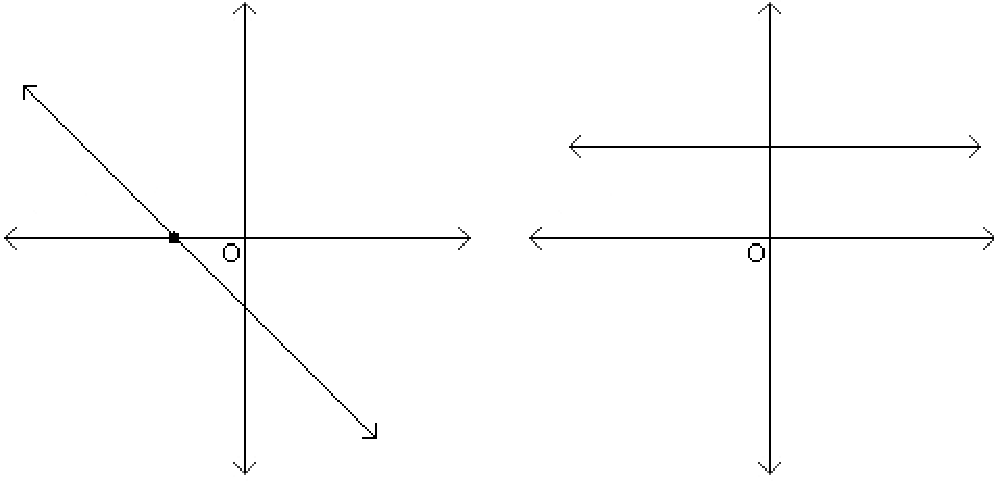
\includegraphics[bb = -40 0 5 250, scale = .5]{line1}

Property $2$ says that two points uniquely determine a line. 

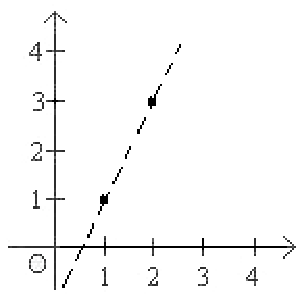
\includegraphics[bb = 0 0 125 145, scale = 0.7]{line3}


\subsection*{ Polynomial Interpolation}
 
Property $2$ says that two points uniquely determine a degree $1$ 
polynomial (a line), three points uniquely determine a degree $2$ 
polynomial, four points uniquely determine a degree $3$ polynomial, 
and so on.  Given $d+1$ pairs $(x_1, y_1), \ldots, (x_{d+1}, y_{d+1})$,
how do we determine the polynomial $p(x) = a_d x^d + \ldots + a_1 x + a_0$
such that $p(x_i) = y_i$ for $i = 1$ to $d+1$? We will give an efficient algorithms for reconstructing the coefficients
$a_0, \ldots, a_d$, and therefore the polynomial $p(x)$. 

The method is called {\em Lagrange interpolation}:
Let us start by solving an easier problem. Suppose that we 
are told that $y_1 =1$ and $y_j = 0$ for $2 \leq j \leq d+1$. Now 
can we reconstruct $p(x)$? Yes, this is easy! Consider 
$q(x) = (x - x_2)(x - x_3) \cdots (x-x_{d+1})$. This is a 
polynomial of degree $d$ (the $x_i$'s are constants, and 
$x$ appears $d$ times). Also, we clearly have
$q(x_j) = 0$ for $2 \leq j \leq d+1$.  But what is $q(x_1)$? 
Well, $q(x_1) = (x_1 - x_2)(x_1 - x_3) \cdots (x_1 - x_{d+1})$,
which is some constant not equal to~$0$. 
Thus if we let $p(x) = q(x)/q(x_1)$ (dividing is ok since 
$q(x_1) \neq 0$), we have the polynomial we are looking for.
For example, suppose you were given the pairs $(1,1)$, $(2,0)$, and
$(3,0)$. Then we can construct the degree $d = 2$ polynomial $p(x)$ by letting
$q(x) = (x - 2)(x - 3) = x^2 - 5x + 6$, and $q(x_1) = q(1) = 2$.
Thus, we can now construct $p(x) = q(x)/q(x_1) = (x^2 - 5x + 6)/2$.

Of course the problem is no harder if we single out some arbitrary 
index $i$ instead of $1$: i.e. $y_i = 1$ and $y_j = 0$ for $j \neq i$. 
Let us introduce some notation: let us denote by $\Delta_i(x)$ 
the degree $d$ polynomial that goes through these $d+1$ points. 
Then $\Delta_i(x) = \frac{\Pi{j\neq i} (x-x_j)}{\Pi{j\neq i} (x_i-x_j)}$.

Let us now return to the original problem. Given 
$d+1$ pairs $(x_1, y_1), \ldots, (x_{d+1}, y_{d+1})$, we 
first construct the $d+1$ polynomials 
$\Delta_{1}(x), \ldots , \Delta_{d+1}(x)$. Now 
we can write $p(x) = \sum_{i = 1}^{d+1} y_i \Delta_i(x)$.
Why does this work? First notice that $p(x)$ is a polynomial 
of degree $d$ as required, since it is the sum of polynomials 
of degree $d$. And when it is evaluated at $x_i$, $d$ of the 
$d+1$ terms in the sum evaluate to $0$ and the $i$-$th$ term 
evaluates to $y_i$ times $1$, as required. 

As an example, suppose we want to find the degree-2 polynomial $p(x)$
that passes through the three points $(1,1)$, $(2,2)$ and $(3,4)$.
The three polynomials~$\Delta_i$ are as follows:
If $d = 2$, and $x_i = i$, for instance, then
\begin{align*}
\Delta_1(x) &= \frac{(x - 2)(x - 3)}{(1 - 2)(1 - 3)} = \frac{(x - 2)(x - 3)}{2} = \frac{1}{2}x^2 - \frac{5}{2}x + 3;\\
\Delta_2(x) &= \frac{(x - 1)(x - 3)}{(2 - 1)(2 - 3)} = \frac{(x - 1)(x - 3)}{-1} = -x^2 +4x -3;\\
\Delta_3(x) &= \frac{(x - 1)(x - 2)}{(3 - 1)(3 - 2)} = \frac{(x - 1)(x - 2)}{2} = \frac{1}{2}x^2 -\frac{3}{2}x +1.
\end{align*}
The polynomial $p(x)$ is therefore given by $$
  p(x) = 1\cdot\Delta_1(x) + 2\cdot\Delta_2(x) + 4\cdot\Delta_3(x) = \frac{1}{2}x^2 -\frac{1}{2}x +1.  $$
You should verify that this polynomial does indeed pass through the above three points.

\subsubsection*{Proof of Property 2}

We would like to prove property ~2:

\noindent
{\bf Property 2:} Given $d+1$ pairs $(x_1, y_1), \ldots, (x_{d+1}, y_{d+1})$,
with all the $x_i$ distinct, 
there is a unique polynomial $p(x)$ of degree (at most) $d$ such that
$p(x_i) = y_i$ for $1 \leq i \leq d+1$.

We have shown how to find a polynomial $p(x)$ such that $p(x_i) = y_i$
for $d+1$ pairs $(x_1,y_1),\dots,(x_{d+1},y_{d+1})$.
This proves part of property~2 (the existence of the polynomial).  How do
we prove the second part, that the polynomial is unique? 
Suppose for contradiction that there is another polynomial $q(x)$ such that $q(x_i) = y_i$
for all $d+1$ pairs above. 
Now consider the polynomial $r(x) = p(x) - q(x)$. Since we are assuming that $q(x)$ and $p(x)$
are different polynomials, $r(x)$ must be a non-zero polynomial of degree at most $d$. 
Therefore, property 1 implies it can have at most $d$ roots.
But on the other hand $r(x_i) = p(x_i) - q(x_i) = 0$ on $d+1$ distinct
points. Contradiction. Therefore, $p(x)$ is the unique polynomial that
satisfies the $d+1$ conditions.

\subsection*{Polynomial Division}
Let's take a short digression to discuss polynomial division,
which will be useful in the proof of property~1. 
If we have a polynomial $p(x)$ of degree $d$, we can divide by 
a polynomial $q(x)$ of degree $\leq d$ by using long division. The result will be:
$$
p(x) = q(x)q'(x) + r(x)
$$

where $q'(x)$ is the quotient and $r(x)$ is the remainder. The degree of $r(x)$ must
be smaller  than the degree of $p(x)$.

\textbf{Example.}
We wish to divide $p(x) = x^3 + x^2 - 1$ by $q(x) = x - 1$: 

\polylongdiv{X^3 + X^2 -1}{X-1}
 
 Now $p(x) = x^3 + x^2 - 1 = (x-1)(x^2 + 2x + 2) +  1$, $r(x) = 1$ and $q'(x) = x^2 + 2x + 2$. 
\subsection*{Proof of Property 1}

Now let us turn to property~1: a non-zero polynomial of degree $d$ has at most $d$
roots.The idea of the proof is as follows.
We will prove the following claims:
\begin{itemize}
\item[]{\bf Claim 1} If $a$ is a root of a polynomial $p(x)$ with degree $d$, 
then $p(x) = (x-a)q(x)$ for a polynomial $q(x)$ with degree $d-1$. 
\item[]{\bf Claim 2} A polynomial $p(x)$ of degree $d$ with distinct roots $a_1,\dots,a_d$ can be
written as $p(x) = c(x-a_1)\cdots(x-a_d)$. 
\end{itemize}
Claim 2 implies property 1. We must show that $a \neq a_i$ for $i = 1, \ldots d$ cannot be a root of $p(x)$.
But this follows from claim 2, since $p(a) = c(a-a_1)\cdots(a-a_d) \neq 0$. 

\subsubsection*{Proof of Claim 1}

Dividing $p(x)$ by $(x-a)$ gives
$p(x) = (x-a)q(x) + r(x)$, where $q(x)$ is the quotient and
$r(x)$ is the remainder. The degree of $r(x)$ is necessarily
smaller than the degree of the divisor $(x-a)$. Therefore
$r(x)$ must have degree $0$ and therefore is some constant $c$.
But now substituting $x=a$, we get $p(a) = c$. But since $a$ is
a root, $p(a) = 0$. Thus $c= 0$ and therefore $p(x) = (x-a)q(x)$,
thus showing that $(x-a)|p(x)$.

\subsubsection*{Claim 1 implies Claim 2}

Proof by induction on $d$.  
\begin{itemize}
\item Base Case: We must show that a polynomial $p(x)$ of degree 1 with root $a_1$ can be written as $p(x)
 = c(x-a_1)$. By Claim 1, we know that
$p(x) = (x-a_1)q(x)$, where $q(x)$ has degree 0 and is therefore a constant. 
\item Inductive Hypothesis: A polynomial of degree $d-1$ with distinct roots $a_1,\dots,a_{d-1}$ can 
be written as $p(x) = c(x-a_1)\cdots(x - a_{d-1})$. 
\item Inductive Step: Let $p(x)$ be a polynomial of of degree $d$ with distinct roots
$a_1,\cdots,a_d$. By Claim 1, $p(x) = (x-a_d)q(x)$ for some polynomial $q(x)$ of degree $d-1$. Since $0 = p(a_i) = 
(a_i-a_d)q(a_i)$ for all $i\neq d$  and $a_i-a_d \neq 0$ in this case, $q(a_i)$ must be equal 
to 0. Then $q(x)$ is a polynomial of degree
$d-1$ with distinct roots $a_1,\dots,a_{d-1}$. We can
now apply the inductive assumption to $q(x)$ to write $q(x) = c(x-a_1)\cdots(x - a_{d-1})$. 
Substituting in $p(x) = (x-a_d)q(x)$, we finally obtain that 
$p(x) = c(x-a_1)\cdots(x-a_d)$.  
\end{itemize}


\section*{Finite Fields}

Both property 1 and property 2 also hold when the values of the 
coefficients and the variable $x$ are chosen from the complex 
numbers instead of the real numbers or even the rational numbers. 
They do not hold if the values are restricted to being natural 
numbers or integers. Let us try to understand this a little more 
closely. The only properties of numbers that we used in polynomial 
interpolation and in the proof of property 1 is that we can 
add, subtract, multiply and divide any pair of numbers as long
as we are not dividing by $0$. We cannot subtract two natural 
numbers and guarantee that the result is a natural number. And 
dividing two integers does not usually result in an integer. 

But if we work with numbers modulo a prime $m$, then we can 
add, subtract, multiply and divide (by any non-zero number modulo $m$).
To check this, recall that $x$ has an inverse mod~$m$ if $\gcd(m,x)=1$,
so if $m$ is prime {\it all\/} the numbers $\{1,\ldots,m-1\}$
have an inverse mod~$m$.
So both property 1 and property 2 hold if the coefficients and 
the variable $x$ are restricted to take on values modulo $m$. 
This remarkable fact that these properties hold even when we 
restrict ourselves to a {\em finite} set of values is the key to
several applications that we will presently see. 

Let us consider an example of degree $d = 1$ polynomials modulo $5$.
Let $p(x) = 2x + 3 (\bmod 5)$. 
The roots of this polynomial are all values $x$ such that $2x + 3 = 0 (\bmod 5)$ 
holds. Solving for $x$, we get that $2x = -3 = 2 (\bmod 5)$ or $x = 1 (\bmod 5)$.  
Note that this is consistent with property 1 since we got only 1 root of a degree 1 polynomial. 

Now consider the polynomials $p(x) = 2x + 3$ and $q(x) = 3x-2$ with all numbers reduced mod $5$. 
We can plot the value of each polynomial $y$ as a function of $x$ in the $x$-$y$ plane. 
Since we are working modulo $5$, there are only $5$ possible choices for $x$, and only $5$ possible choices for $y$:

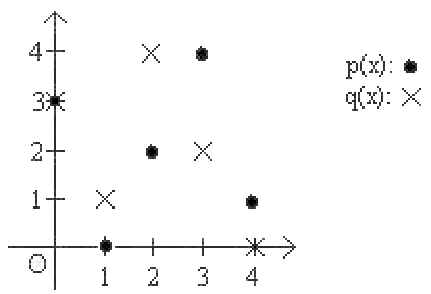
\includegraphics[bb = 0 0 140 143, scale = 0.7]{graph2}

Notice that these two ``lines" intersect in exactly one point,
even though the picture looks nothing at all like lines in 
the Euclidean plane! Looking at these graphs it might seem remarkable that both property 1 and property 2 hold
when we work modulo $m$ for any prime number $m$. But as we stated above, 
all that was required for the proofs of property 1 and 2
was the ability to add, subtract, multiply and divide any pair of numbers 
(as long as we are not dividing by 0), and they hold whenever we work modulo a prime $m$. 

When we work with numbers modulo a prime $m$, we say that we are working over a
finite field, denoted by $F_m$ or $GF(m)$ (for Galois Field). In order
for a set to be called a field, it must satisfy certain axioms which are
the building blocks that allow for these amazing properties and others to hold.
If you would like to learn more about fields and the axioms they satisfy,
you can visit Wikipedia's site and read the article on fields:
\url{http://en.wikipedia.org/wiki/Field_\%28mathematics\%29}. While you are there,
you can also read the article on Galois Fields and learn more about some of their
applications and elegant properties which will not be covered in this lecture:
\url{http://en.wikipedia.org/wiki/Galois_field}.



\section*{Counting}

How many polynomials of degree (at most)~$2$ are there modulo $m$? 
This is easy: there are $3$ coefficients, each of which can take on one of $m$
values for a total of $m^3$. Writing $p(x) = a_d x^d + a_{d-1} x^{d-1} + \ldots + a_0$
by specifying its $d+1$ coefficients $a_i$ is known as the coefficient representation 
of $p(x)$. Is there any other way to specify $p(x)$? 

Sure, there is! Our polynomial of degree (at most)~$2$ is uniquely specified by 
its values at any three points, say $x = 0, 1, 2$. Once again each of these three
values can take on one of $m$ values, for a total of $m^3$ possibilities. 
In general, we can specify a degree $d$ polynomial $p(x)$ by specifying its
values at $d+1$ points, say $0, 1, \ldots , d$. These $d+1$ values, $(y_0,y_1, \dots,y_d)$
are called the value representation of $p(x)$. The coefficient representation
can be converted to the value representation by evaluating the polynomial
at $0, 1, \dots, d$. And as we've seen, polynomial interpolation can convert the value
representation to the coefficient representation.

So if we are given three pairs $(x_1, y_1), (x_2,y_2), (x_3, y_3)$ then  
there is a unique polynomial of degree $2$ such that $p(x_i) = y_i$.  
But now, suppose we were only given two pairs 
$(x_1, y_1), (x_2, y_2)$; how many distinct degree $2$ polynomials
are there that go through these two points? Notice
that there are exactly $m$ choices for $y_3$, and for each choice there 
is a unique (and distinct) polynomial
of degree $2$ that goes through the three points $(x_1, y_1), (x_2,y_2), (x_3, y_3)$. 
It follows that there are exactly $m$ polynomials of degree at most $2$ that go
through $2$ points $(x_1, y_1), (x_2, y_2)$, as shown below:

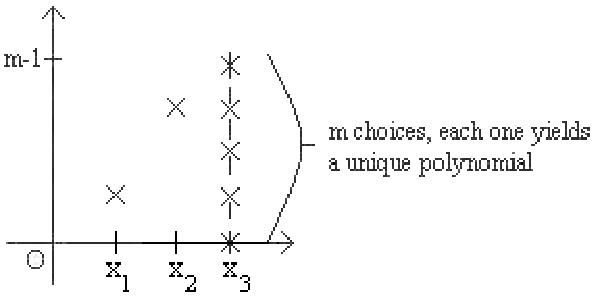
\includegraphics[bb = 0 0 125 147, scale = 0.7]{graph3}

What if you were only given one point $(x_1, y_1)$? Well, there are $m^2$ choices for
$y_2$ and $y_3$, yielding $m^2$ polynomials of degree at most $2$ that go
through the point given. A pattern begins
to emerge, as is summarized in the following table:\\

\begin{tabular}{|c|c|}
\hline
\multicolumn{2}{|c|}{\text{Polynomials of degree $\le d$ over $F_m$}} \\ \hline
\text{\# of points} & \text{\# of polynomials} \\ \hline
$d+1$  & $1$ \\
$d$    & $m$ \\
$d-1$  & $m^2$ \\
\vdots & \vdots \\
$d-k$  & $m^{k+1}$ \\
\vdots & \vdots \\
$0$  & $m^{d+1}$ \\
\hline
\end{tabular} \\

Note that the reason that we can count the number of polynomials in this setting
is because we are working over a finite field. If we were working over an
infinite field such as the rationals, there would be infinitely many
polynomials of degree d that can go through d points! Think of a line,
which has degree one. If you were just given one point, there would be
infinitely many possibilities for the second point, each of which
uniquely defines a line.



\section*{Secret Sharing}
In the late 1950's and into the 1960's, during the Cold War, President
Dwight D. Eisenhower approved instructions and authorized top
commanding officers for the use of nuclear weapons under very urgent
emergency conditions. Such measures were set up in order to defend the
United States in case of an attack in which there was not enough time
to confer with the President and decide on an appropriate response. 
This would allow for a rapid response in case of a Soviet
attack on U.S. soil. This is a perfect situation in which a secret
sharing scheme could be used to ensure that a certain number of
officials must come together in order to successfully launch a nuclear
strike, so that for example no single person has the power and control
over such a devastating and destructive weapon.  Suppose the U.S.\ 
government finally decides that a nuclear strike can be initiated only
if at least $k > 1$ major officials agree to it. We want to devise a
scheme such that (1) any group of $k$ of these officials can pool
their information to figure out the launch code and initiate the
strike but (2) no group of $k - 1$ or fewer have any information about
the launch code, even if they pool their knowledge. For example,
they should not learn whether the secret is odd or even, a prime number,
divisible by some number $a$, or the secret's least significant bit. How
can we accomplish this?

Suppose that there are $n$ officials indexed from $1$ to $n$ and the launch code is some
natural number $s$. Let $q$ be a prime number larger than $n$ and $s$.
We will work over $GF(q)$ from now on.

Now pick a random polynomial $P(x)$ of degree $k - 1$ such that $P(0) = s$ and give
$P(1)$ to the first official, $P(2)$ to the second,\ldots, $P(n)$ to the $n^{th}$. Then
\begin{itemize}

\item Any $k$ officials, having the values of the polynomial at $k$
points, can use Lagrange interpolation to find $P$, and once they know
what $P$ is, they can compute $P(0) = s$ to learn the secret. 
Another way to say this is that any $k$ officials have between them a value representation of the polynomial,
which they can convert to the coefficient representation, which allows them to evaluate $P(0) = s$. 

\item Any group of $k - 1$ officials has no information about~$s$.
So they know only $k-1$ points through which $P(x)$, an unknown polynomial of 
degree $k-1$ passes. They wish to reconstruct $P(0)$. But by our discussion 
in the previous section, for each possible value $P(0) = b$, there is a unique 
polynomial of degree $k-1$ that passes through the $k-1$ points of the $k-1$ officials
as well as through $(0, b)$. Hence the secret could
be any of the $q$ possible values $\{0,1,\ldots,q-1\}$, so the officials
have---in a very precise sense---no information about~$s$. 
Another way of saying this is that the information of the officials is consistent
with $q$ different value representations, one for each possible value of the secret, 
and thus the officials have no information about $s$. 
(Note that
this is the main reason we choose to work over finite fields rather than,
say, over the real numbers, where the basic secret-sharing scheme would
still work.  Because there are only finitely many values
in our field, we can quantify precisely how many remaining possibilities
there are for the value of the secret, and show that this is the same as if
the officials had no information at all.)
\end{itemize}
\textbf{Example.} Suppose you are in charge of setting up a secret
sharing scheme, with secret $s=1$, where you want to distribute 
$n = 5$ shares to $5$ people such that any $k = 3$ or more people can 
figure out the secret, but two or fewer cannot. Let's say we are working 
over $GF(7)$ (note that $7>s$ and $7>n$) 
and you randomly choose the following polynomial of degree 
$k-1 = 2: P(x) = 3x^2 + 5x + 1$ (here, $P(0) = 1 = s$, the secret). 
So you know everything there is
to know about the secret and the polynomial, but what about the people
that receive the shares? Well, the shares handed out are $P(1) =
2$ to the first official, $P(2) = 2$ to the second, $P(3) = 1$ to the third,
$P(4) = 6$ to the fourth, and $P(5) = 3$ to the fifth official. Let's say that officials
3, 4, and 5 get together (we expect them to be able to recover the
secret). Using Lagrange interpolation, they compute the following
delta functions:
\begin{align*}
\Delta_3(x) &= \frac{(x - 4)(x - 5)}{(3 - 4)(3 - 5)} = \frac{(x - 4)(x - 5)}{2} = 4(x-4)(x-5);\\
\Delta_4(x) &= \frac{(x - 3)(x - 5)}{(4 - 3)(4 - 5)} = \frac{(x - 3)(x - 5)}{-1} = 6(x-3)(x-5);\\
\Delta_5(x) &= \frac{(x - 3)(x - 4)}{(5 - 3)(5 - 4)} = \frac{(x - 3)(x - 4)}{2} = 4(x-3)(x-4).
\end{align*}
They then compute the polynomial over $GF(7)$: $P(x) =
(1)\Delta_3(x)+(6)\Delta_4(x)+(3)\Delta_5(x) = 3x^2+5x+1$ (verify the
computation!). Now they simply compute $P(0)$ and discover that the
secret is $1$.

Let's see what happens if two officials try to get together, say persons
1 and 5. They both know that the polynomial looks like $P(x) = a_2x^2 +
a_1x + s$. They also know the following equations:
\begin{align*}
P(1) &= a_2 + a_1 + s = 2\\
P(5) &= 4a_2 + 5a_1 + s = 3
\end{align*}
But that is all they have two equations with three unknowns, and thus they
cannot find out the secret.  This is the case no matter which two
officials get together. Notice that since we are working over $GF(7)$,
the two people could have guessed the secret ($0 \le s \le 6$) and
constructed a unique degree 2 polynomial (by property~2). But the two
people combined have the same chance of guessing what the secret is as
they do individually. This is important, as it implies that two people
have no more information about the secret than one person does.
\end{document}
